\documentclass{article}
\usepackage[a4paper, portrait, margin=1.1811in]{geometry}
\usepackage[english]{babel}
\usepackage[utf8]{inputenc}
\usepackage[T1]{fontenc}
\usepackage{helvet}
\usepackage{etoolbox}
\usepackage{graphicx}
\usepackage{titlesec}
\usepackage{caption}
\usepackage{booktabs}
\usepackage{xcolor} 
\usepackage[colorlinks, citecolor=cyan]{hyperref}
\usepackage{caption}
\captionsetup[figure]{name=Figure}
\graphicspath{ {./images/} }
\usepackage{scrextend}
\usepackage{fancyhdr}
\usepackage{graphicx}
\newcounter{lemma}
\newtheorem{lemma}{Lemma}
\newcounter{theorem}
\newtheorem{theorem}{Theorem}
\usepackage{pdfpages}
\usepackage{subfigure}

\usepackage[nottoc]{tocbibind}
\usepackage[square,numbers]{natbib}
\bibliographystyle{abbrvnat}

%\pagestyle{plain}
\makeatletter
\patchcmd{\@maketitle}{\LARGE \@title}{\fontsize{16}{19.2}\selectfont\@title}{}{}
\makeatother

\usepackage{authblk}
\renewcommand\Authfont{\fontsize{10}{10.8}\selectfont}
\renewcommand\Affilfont{\fontsize{10}{10.8}\selectfont}
\renewcommand*{\Authsep}{, }
\renewcommand*{\Authand}{, }
\renewcommand*{\Authands}{, }
\setlength{\affilsep}{2em}  
\newsavebox\affbox
\author[1]{\textbf{Yongye Tan}}

\titlespacing\section{0pt}{12pt plus 4pt minus 2pt}{0pt plus 2pt minus 2pt}
\titlespacing\subsection{12pt}{12pt plus 4pt minus 2pt}{0pt plus 2pt minus 2pt}
\titlespacing\subsubsection{12pt}{12pt plus 4pt minus 2pt}{0pt plus 2pt minus 2pt}


\titleformat{\section}{\normalfont\fontsize{10}{15}\bfseries}{\thesection.}{1em}{}
\titleformat{\subsection}{\normalfont\fontsize{10}{15}\bfseries}{\thesubsection.}{1em}{}
\titleformat{\subsubsection}{\normalfont\fontsize{10}{15}\bfseries}{\thesubsubsection.}{1em}{}

\titleformat{\author}{\normalfont\fontsize{10}{15}\bfseries}{\thesection}{1em}{}

\title{\textbf{\huge Absenteeism at Work}}
\date{}    

\begin{document}

\pagestyle{headings}	
\newpage
\setcounter{page}{1}
\renewcommand{\thepage}{\arabic{page}}


	
\captionsetup[figure]{labelfont={bf},labelformat={default},labelsep=period,name={Figure }}	\captionsetup[table]{labelfont={bf},labelformat={default},labelsep=period,name={Table }}
\setlength{\parskip}{0.5em}
	
\maketitle


\section{Introduction}
In the modern world, it is common to see people be absent from work for various reasons. Absenteeism at a workplace affects the accountability and availability of a person, leads to negative consequences in a team or a company such as the decline in work reputation, and the decrease in work coordination across departments. In this report, we are analyzing an existing dataset, from Kaggle \cite{wagner_2019}, records of absenteeism at work from July 2007 to July 2010 at a courier company in Brazil \cite{vulpen_2021}. There are 740 observations and 21 variables. Important variables exist such as Distance from Residence to Work, Work load Average/day, which are important factors to determine why a worker is absent.
The central question in this article is: What is the main determinant of whether someone is absent or not from work?


\section{Overview of the data set}
To know more about the 21 variables in this dataset, the name of all the variables is given below: Month of absence; Day of the week; Seasons; Transportation expense; Distance from Residence to Work in kilometers; Service time; Age; Work load Average/day; Hit target; Disciplinary failure; Education; the number of children; Social drinks; Social smoker; Pet; Weight; Height; Body mass Index (BMI); Absenteeism times in hours. \
\textbf{Note:} Disciplinary failure, Social drink and smoker are binary variables, meaning yes = 1 and no = 0. In Day of the week, Monday, Tuesday, Wednesday, Thursday and Friday represents as 2, 3, 4, 5 and 6, respectively.



\section{Exploratory Analysis}
In order to answer this central question, we will explore the dataset first and then break it down to sub-questions. Here are the procedures to exploring the data:
\begin{itemize}
  \item Data Clean up
  \item Explore important variables such as Absenteeism.time.in.hours. and Education
  \item Ask specific questions regarding various factors
\end{itemize}

There are zero NA or missing value in every row, meaning the data is clean. Since the data contains no missing value, we can start exploring variables. The average time of absence in hours per week is 6.924 hours, and the maximum is 120 hours -- a worker was absent for a whole week from Monday to Friday. We are interested of knowing the distributions of worker with various degrees. We found that there are 611, 46, 79, and 4 workers with high school, graduate, post-graduate, and master and doctor degrees, respectively. The potential factors that cause a worker to be a absent are distance, workload, day of week or month of year. Here are the sub-questions I want to explore and discuss to answer the central question: 
\begin{enumerate}
    \item How does amount of workload affect the absenteeism as a person ages?
    \item Is there a specific day of a week or month of a year absenteeism occurs the most?
    \item Does bad habits lead to not showing up to work?
    \item How does distance from work have an effect on workers to commute to their workplace?
\end{enumerate}


\section{Discussion}
To answer the first question, we need to explore the relationship between age and workload. Figure 1 is a scatter-plot graph for average amount of workload across age 27 to 58. Outliers are normal since certain age group works more than others. We find that a worker tends to work more towards age 30 and 40, and have a decline trend of working less and less after age 42 (indicated by the dotted vertical red line). There are 274, 263 and 249 workloads at age 28, 47, and 59, respectively. This is understandable because human lose the tendency to work longer and harder as one gets older since their physical body lose the ability to support long shifts or heavy duty. To take a look further, we explore the relationship between age and the hours of absent per week across ages in Figure 2. We find that old age associates with longer absent time, young age associates with shorter absent time. At age 29, the average absent time is 4.43 hours, whereas at age 46 is 8.00 hours. Therefore, workload is negatively associated with age, and absent time is positively associated with age. In conclusion, as a person gets older, the less workload he/she receives, leading to a higher chance of being absent in the workplace and getting ready to retire.
\begin{figure}[h]
 \centering
 \begin{minipage}[b]{.5\textwidth}
  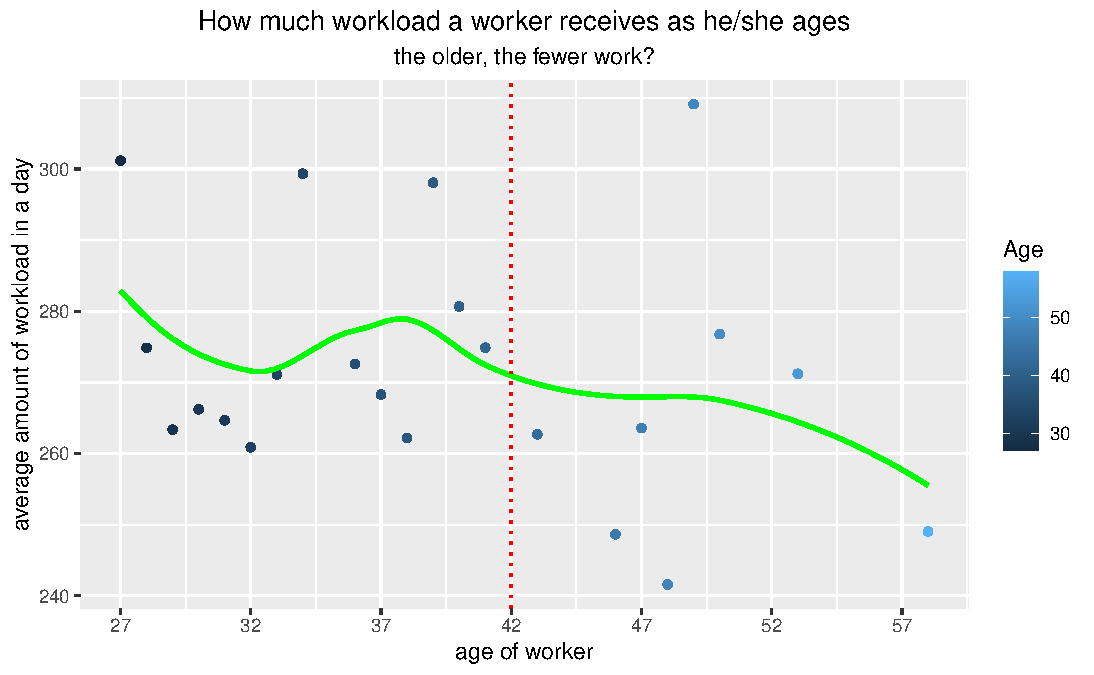
\includegraphics[width=1\linewidth]{age_workload.pdf}
  \caption{workload across ages}
 \end{minipage}
% \qquad
 \begin{minipage}[b]{.4\textwidth}
  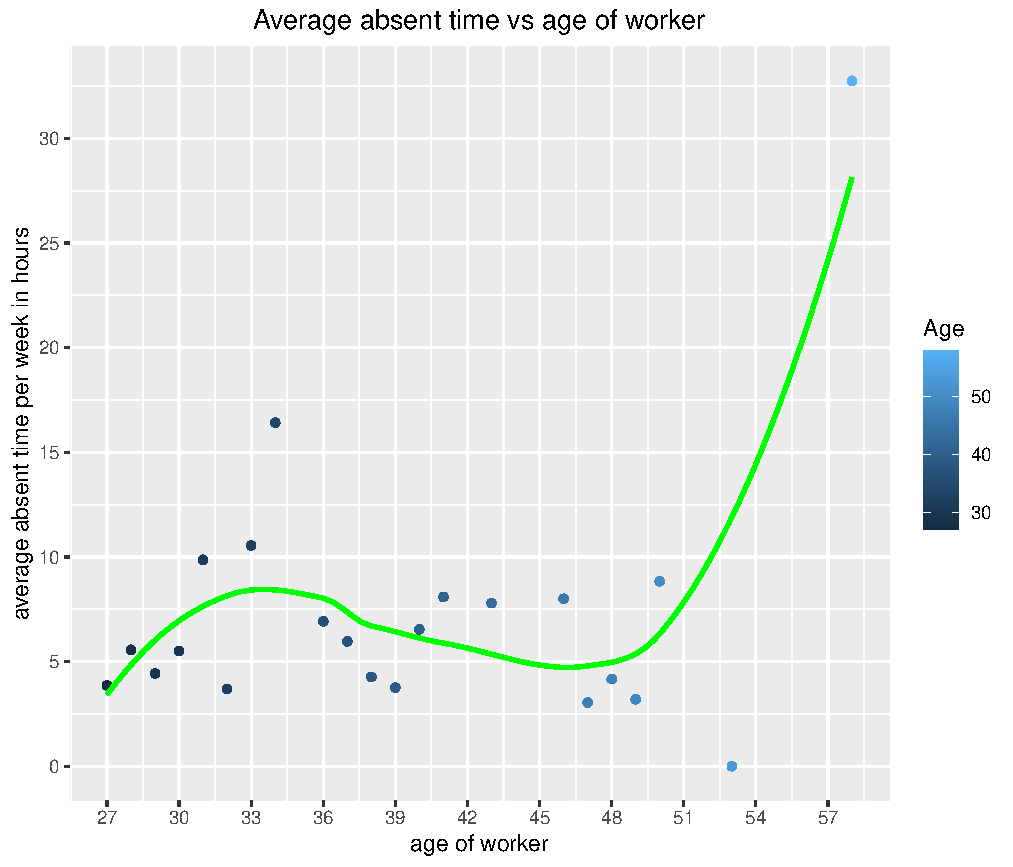
\includegraphics[width=1\linewidth]{absentTime_age.pdf}
  \caption{absent time across ages}
 \end{minipage}
\end{figure}

Generally, people have different feelings of working on different days of a week. According to an article from insidehook, there is a quote saying "No one wants to work on a Friday afternoons anymore. If the task at hand can be pushed back to Monday, or next week, then that’s the option everyone’s going to agree on". Workers tend to be more relaxed and decides to give themselves a small break on Friday afternoon and push their work to next week. If that is the case, we would like to analyze the absent statistics from Monday to Friday from our dataset.
\begin{figure}[h]
 \centering
 \begin{minipage}[b]{.4\textwidth}
  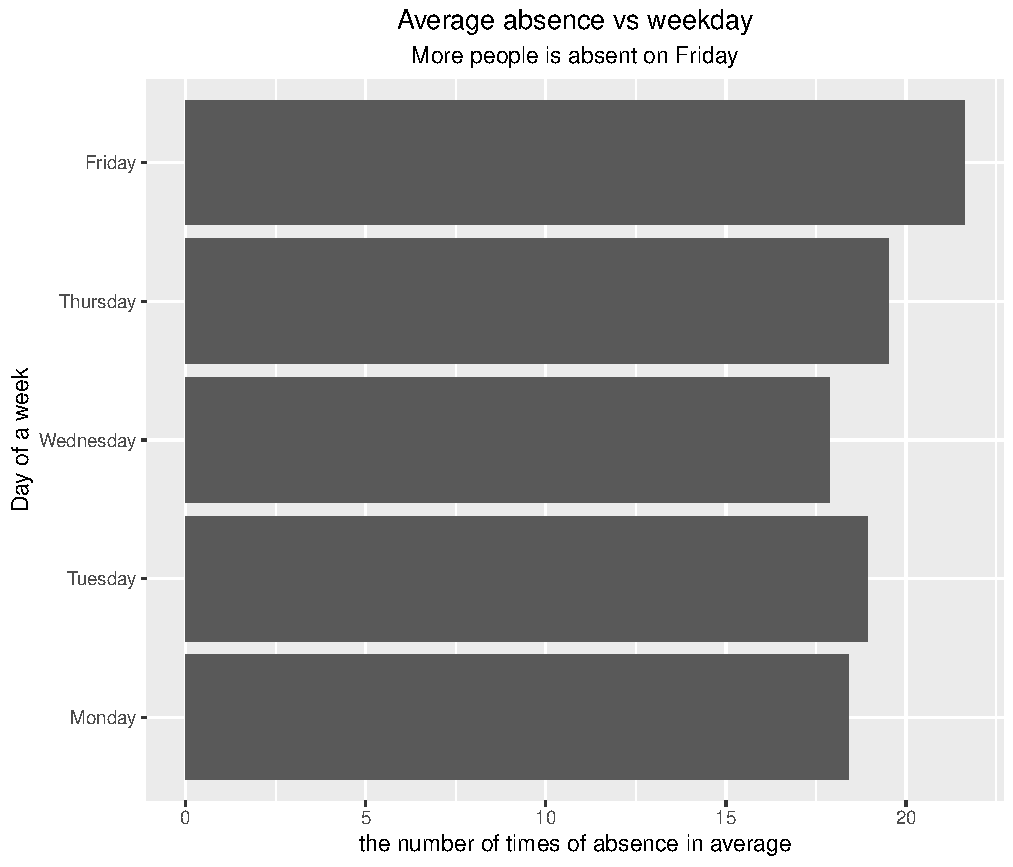
\includegraphics[width=1\linewidth]{absent_workday.pdf}
  \caption{Absent across days}
 \end{minipage}
% \qquad
 \begin{minipage}[b]{.4\textwidth}
  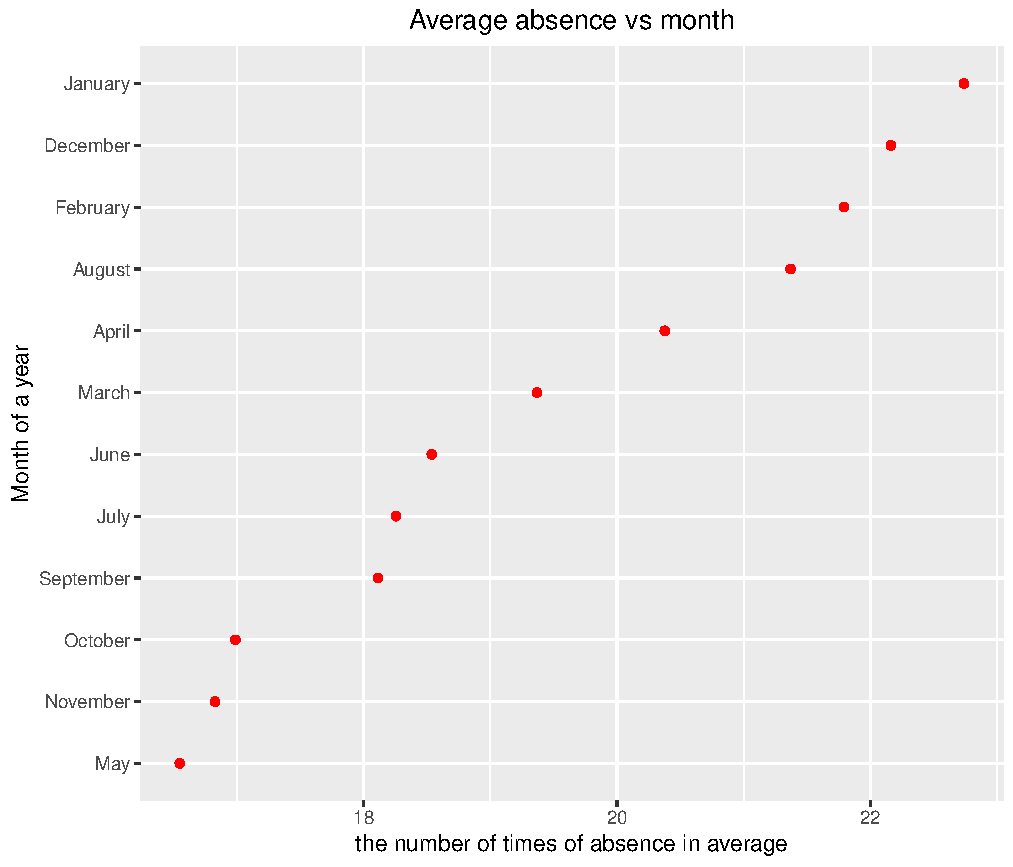
\includegraphics[width=1\linewidth]{absent_month.pdf}
  \caption{Absent across months}
 \end{minipage}
\end{figure}
Figure 3 is a bar graph for the number of times of absence in average per week from Mon. to Fri.. We find that Friday has the most absence, which is 21.6 hours, Thursday has the second most absence, which is 19.5 hours, and Wednesday has the lowest absence, which is 17.9 hours. This adds more evidence to the argument from the article that more people are absent on Fridays. Since the day of a week has an effect on the absenteeism, we would also want to investigate whether the month of a year would also have a similar affect. Figure 4 is a scatter-plot graph showing the relationship between the number of times of absence in average in 12 months. The months have been sorted based on the number of absence, not by the order of months. From figure 4, January is placed at the top of the y-axis, as it has the most absence in average, which is 22.7 hours per week, whereas May has the least absence, which is 16.5 hours per week. January, December, February, August, are the most, second most, third most, and fourth most absence months in the dataset. These months are associated with vacations and holidays. There are Christmas, New Year's Day, and winter vacation between December and February, and summer vacation in August. This is intuitive because workers spend more time with families, friends, or themselves during holiday and vacation after working for long months at the workplace. Figure 4 also illustrates to us that workers do not get much absence in May, October, and November, which might be an indication that they want to work hard towards the end of the season or holiday to improve their performance to gain higher status and reputation within the department or company \cite{maroney_2017}. Therefore, certain months of a year and day of a week would have a higher absence rate in average caused by individual feelings and external holidays. \\

Bad habits prevent us from accomplishing our goals, and have a negative influence on us physically and mentally. We want to explore whether smoking, drinking, and disciplinary failure makes a person less likely to show up to work. We will use T-test \cite{team_2021} to calculate t-statistic, p-value \cite{[mcleod_1970}, and degree of freedom (df), and use them to determine whether our results are statistically significant. If the t-statistic is greater than +2 or less than -2, then this is an indication that it is with great confidence that our prediction is reliable (the higher, the better). If the p-value is less than or equal to 0.05, then null hypothesis is considered as statistically significant; otherwise, it is not statistically significant. Also, the higher the df, the distribution of the graph becomes more of a standard normal distribution, and tells us that the analysis we run is more significant. In this report, I perform the independent 2-group T-test on these binary variables between Social.smoker, Social.drinker, and Disciplinary.failure and Absenteeism.time.in.hours. I found out the t-values are 0.31204, -1.7895, and 14.239, respectively, and p-values are 0.756, 0.07396, 2.2e-16, respectively, and df-values are 69.044, 710.21, and 699, respectively. The only variable that has an extremely small p-value and also less than 0.05 is Disciplinary failure. Not only does it have a small p-value, it also has a high t-value, which tells us that prediction is reliable and the analysis is predictive and df is also significant. Therefore, disciplinary failure is statistically significant on absenteeism in workplace. Example of disciplinary failure includes misuse of social media, email, or criminal conduct. \cite{cosentino_2022}
\begin{figure}[h]
 \centering
 \begin{minipage}[b]{.5\textwidth}
  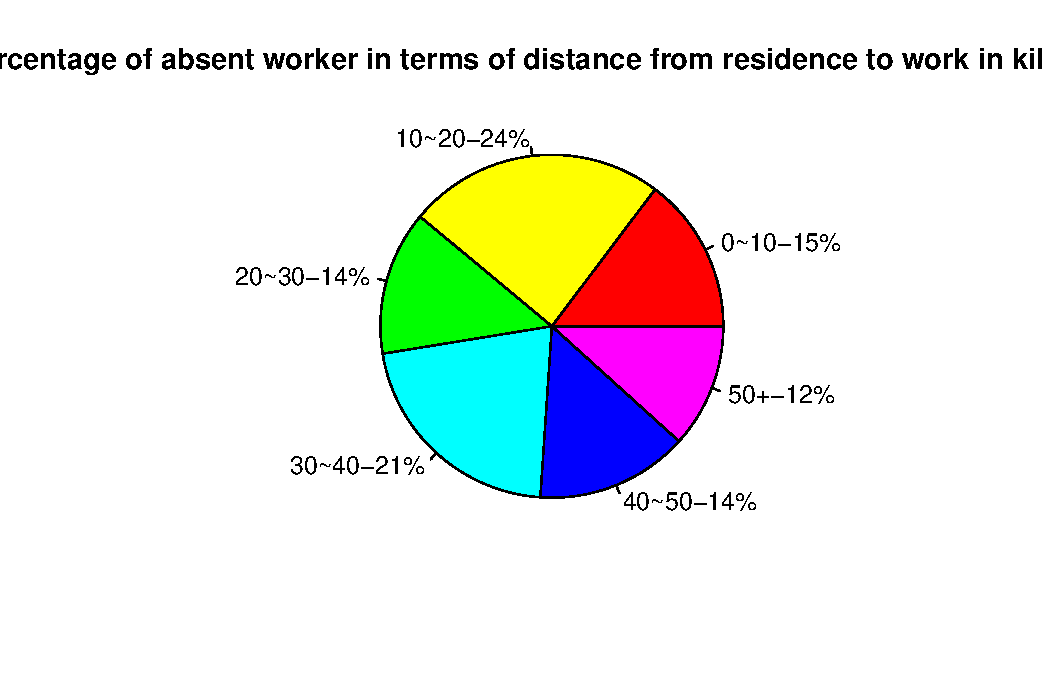
\includegraphics[width=1\linewidth]{pie_distribution.pdf}
  \caption{A pie chart showing the percentage of absent worker who live every 10 km away from office in kilometer}
 \end{minipage}
\end{figure}

Would distance be a reason that makes a worker show up late or not come to work? Intuitively, if a person lives really far away from their workplace, he/she would need to wake up super early and get ready to commute to work. To answer the last question, we need to explore the relationship between distance from residence to work in kilometer and absenteeism in hours per week. Figure 5 is a pie-chart showing the percentage of workers who live every 10 km away from the office. There are 6 slices with the closest from 0 to 10 km and furthest from more than 50 km. We find that the slice with the highest percentage are the ones who lives 10 - 20 km away from their office, and the slice with the lowest percentage are the ones who live 50km+ away. This is understandable because a person who lives far away would be more considerate of their time and try their best to show up to work on time. To investigate this further, we categorize 0-20km as "relatively close", 20-40 as "moderately close", and 40+ as "extremely far". We find that the percentage of "relatively close" is 39\%, "moderately close" is 35\%, "extremely far" is 26\%. There is a decent amount of decline of absent rate as distance increases. Therefore, workers who live closer to their workplace tend to be more absent than those who live further away. This can be explained by psychology as we will not discuss in this paper.

\section{Summary}

After exploring four different questions, we found out absenteeism are not exclusively caused by one factor. The determinant of whether someone is absent or not can be found from the conclusions we draw from the 4 sub-questions with current dataset: 
\begin{enumerate}
    \item As a person gets older, the less workload one receives, the higher chance of absenteeism.
    \item Worker has the highest absenteeism on Fridays, December, January, February, and August.
    \item Disciplinary failure is statistically significant on absenteeism in workplace.
    \item Worker who lives closer to workplace is more absent than those who live further away.
\end{enumerate}
In simple words, we have found that age, time, disciplinary, and distance play a role of the absent rate. This paper covers all the potential and useful variables that can possibly visualize and predict the overall absenteeism in workplace in this particular sample; however, it is not strong enough to elaborate the absenteeism status in a population as our statistical techniques are not strong and enough to support that.


\bibliography{mybib}

\end{document}

